\chapter{Allineamento multi-modale per istologia}
\frenchspacing
\label{chap:histology}
\noindent L'istologia è il ramo delle discipline biologiche che studia la struttura microscopica e ultramicroscopica dei tessuti e degli organi animali e vegetali dal punto di vista morfologico, istochimico e delle attività funzionali da essi applicate~\cite{Istologia}.Tipicamente, si parte dalla analisi di un campione biologico o tessuto prelevato da paziente e tramite una sequenza di operazioni di preparazione si conducono analisi microscopiche per studiarne le caratteristiche normo-patologiche ed identificare malattie o problematiche in generale.
\section{Preparazione istologica}
La preparazione istologica è basata su 5 step fondamentali:
\begin{enumerate}
    \item Fissazione
    \item Disidratazione
    \item Inclusione
    \item Sezionamento
    \item Colorazione
\end{enumerate} \hfill \break
\noindent Il primo passo per produrre un campione istologico è quello della fissazione. Questa procedura è essenziale poiché comprende tecniche di conservazione del tessuto, tecniche atte a rafforzare la struttura cellulare ed infine una valutazione approfondita del campione per determinare se dev'essere esposto ad antigeni, in dipendenza dallo scopo per il quale è stato acquisito dello studio per il quale è stato acquisito~\cite{Alturkistani2015-bz}. \hfill \break
\noindent I fissativi più comuni sono a base di formaldeide, come ad esempio la formalina neutra tamponata (NBF) adoperata per preservare i tessuti o la paraffin-formalina (PFA) adoperata nel contesto dell'immunoistochimica.
A seguito della fissazione si procede con la disidratazione fatta tipicamente tramite etanolo, e la rimozione dell'alcol tramite xylene. Questa serie di operazioni serve a preparare i tessuti e rendere semplice la fase di sezionamento. \hfill \break
\noindent L'ultimo passaggio prima del sezionamento è quella dell'inclusione, che viene effettuata di solito tramite paraffina. Questo processo può portare ad un deterioramento delle cellule, a causa della prolungata esposizione al calore, e per evitare che ciò accada si congelano i tessuti dopo questa fase. \hfill \break
\noindent La fase di sezionamento concerne la preparazione di sezioni mediante microtomo. Le sezioni ottenute sono generalmente, molto sottili perché la luce dei microscopi possa passarci attraverso e permettere l'analisi da parte del ricercatore o specialista.
L'ultima fase è quella della colorazione ed andremo ad analizzarla in dettaglio nella prossima sezione.
\section{Co-registrazione multi-modale}
\noindent Durante la preparazione di un campione istologico vengono tipicamente usate più colorazioni per rivelare proprietà distinte del tessuto o di differenti componenti dello stesso. A causa dei lavaggi, e dei vari processi utili a completare ogni singola colorazione, il tessuto stesso viene però tipicamente deformato ed è richiesta quindi una registrazione non rigida delle varie immagini poi acquisite per poter procedere con una analisi globale del campione~\cite{9058666}.\hfill \break
\noindent Definiamo quindi con il termine ``registrazione multi-modale'' l'acquisizione e successivo allineamento di immagini provenienti dallo stesso campione ma che presentano delle differenze in termini di marcatura/colorazioni. Un esempio di queste marcature differenti è mostrato nelle \Cref{fig:1,fig:2,fig:3,fig:4} che rappresentano immagini, per la maggior parte acquisite in fluorescenza. L'immagine \Cref{fig:1} è stata colorata con Cy3, o Cianina, colorante visibile anche occhio nudo, che mette in evidenza il citoplasma della cellula.
Per la \Cref{fig:2}, è stato usato il DAPI, o ``4', 6-diamidin-2-fenilindolo'', è utile ad evidenziare i nuclei, per la \Cref{fig:3} il FITC, o Isotiocianato di fluoresceina, per le membrane ed infine \Cref{fig:4} usando la luce classica. \par
\noindent 
\begin{figure}[H]
    \centering
    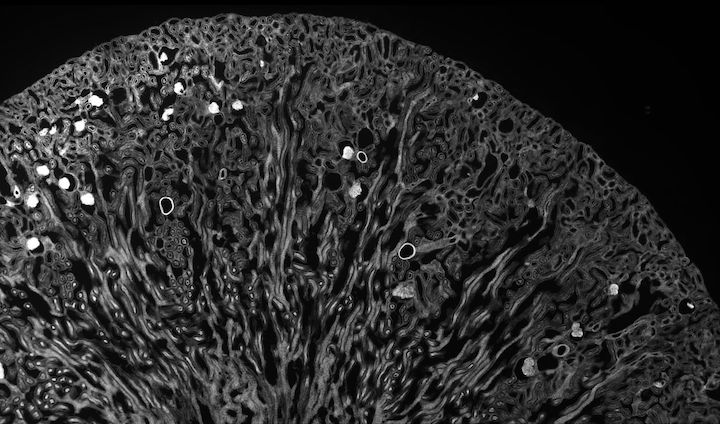
\includegraphics[scale=0.5,keepaspectratio]{multimodal/20190311_Mosaic_Cy3_NoAligned.jpg}
    \caption{Esempio di campione colorato con Cy3}
    \label{fig:1}
\end{figure}
\begin{figure}[H]
    \centering
    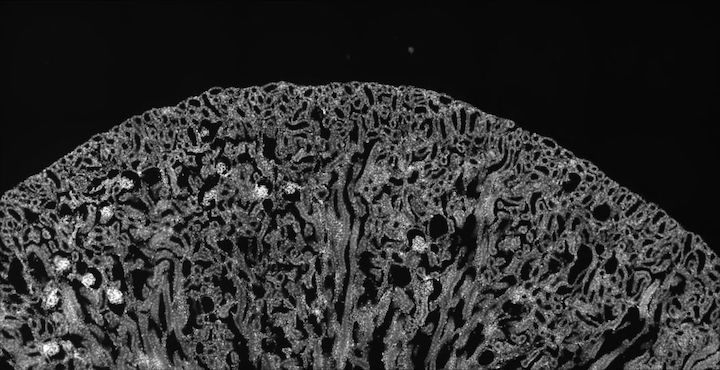
\includegraphics[scale=0.5,keepaspectratio]{multimodal/20190311_Mosaic_DAPI_NoAligned.jpg}
    \caption{Esempio di campione colorato con DAPI}
    \label{fig:2}
\end{figure}
\begin{figure}[H]
    \centering
    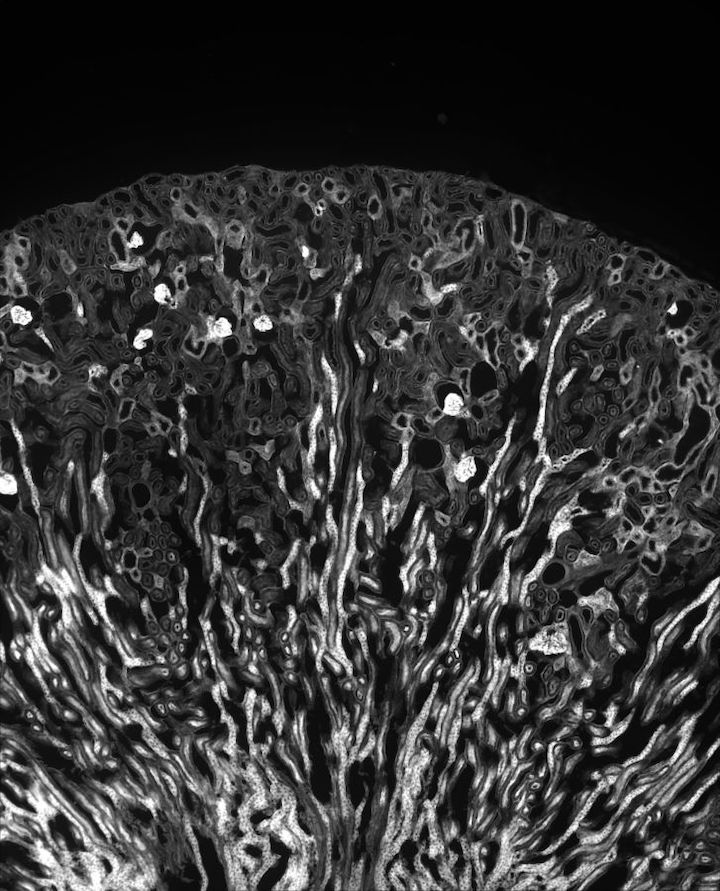
\includegraphics[scale=0.5,keepaspectratio]{multimodal/20190311_Mosaic_FITC_NoAligned.jpg}
    \caption{Esempio di campione colorato con FITC}
    \label{fig:3}
\end{figure}
\begin{figure}[H]
    \centering
    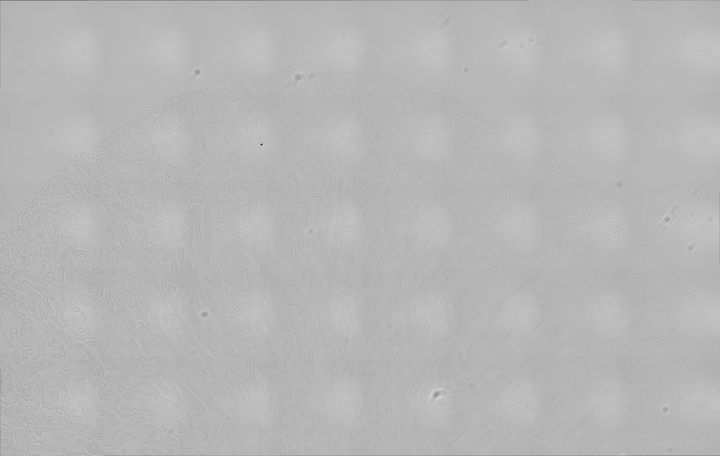
\includegraphics[scale=0.5,keepaspectratio]{multimodal/20190311_Mosaic_DICn2_NoAligned.jpg}
    \caption{Esempio di campione sottoposto a luce classica}
    \label{fig:4}
\end{figure}
\section{Algoritmi di co-registrazione automatica}
\noindent Per poter portare a compimento la co-registrazione multi-modale occorre utilizzare algoritmi di \textit{Computer Vision} in grado di occuparsi di questi cinque punti:
\begin{enumerate}
	\item Rilevamento delle caratteristiche salienti dell'immagine; 
	\item Definizione della corrispondenza delle caratteristiche tra diverse immagini;
	\item Rilevamento delle anomalie;
	\item Derivazione della funzione di trasformazione; 
	\item Ricostruzione dell'immagine finale.
\end{enumerate}
\noindent Chiariamo preventivamente che quando si utilizza il termine \textit{descrittore} si fa riferimento al contenitore che altro non è che il contenente di tutte le informazioni ottenute dopo l'elaborazione di un immagine. Di seguito descriveremo brevemente alcuni esempi di algoritmi noti per la registrazione di immagini, partendo da algoritmi, datati e dispendiosi in termini di risorse, fino a raggiungere quelli più recenti e performanti. \par
\subsection{SIFT - Scale Invariant Feature Transform}
\noindent L'algoritmo \textit{``SIFT''} (\textit{Scale Invariant Feature Transform}) è stato realizzato da D.G. Lowe nel 1999~\cite{Lowe2004}. Il rilevamento di corrispondenze tra immagini, è basato sull'algoritmo chiamato \textit{``Differenze di Gaussiane''}, abbreviato con l'acronimo DoG. Le DoG sono usate per trovare i punti d'interesse invarianti rispetto alla scala e all'orientamento. Per ogni agglomerato di punti si ricerca un modello adatto a determinarne posizione e scala, definendo punti chiave basati sulla stabilità delle loro misurazioni. Per ogni punto chiave viene assegnato un orientamento, in base alla direzione del gradiente locale dell'immagine. I gradienti locali delle immagini vengono misurati ad una scala selezionata, e vengono trasformati in una rappresentazione che permette di considerare cambi d'illuminazione e distorsione della forma.\hfill \break
\noindent La rappresentazione spazio-scala di un immagine è definita da una funzione L(x, y, \(\sigma\)) che è prodotta dalla convoluzione di una variabile spazio-scala Gaussiana G con un immagine in input I~\cite{Lowe2004}. \par
\begin{equation}
	L(x, y, \sigma) = G(x, y, \sigma) * I(x, y)
\end{equation}
\noindent dove la funzione G è definita da:
\begin{equation}
    G(x, y, \sigma) = \frac{1}{2\pi\sigma^2}\euler^\frac{-(x2+y2)}{2\sigma^2}
\end{equation}
\noindent
Al fine di individuare le collocazioni dei punti chiave stabili nella rappresentazione spazio-scala, esprimiamo una funzione D(x, y, \(\sigma\)) e calcoliamo la correlazione tra due scale vicine, facendo la differenza applicando al primo una costante moltiplicativa k:
\begin{equation}
	D(x, y, \sigma) = (G(x, y, k\sigma) - G(x, y, \sigma)) * I(x, y)
\end{equation}
\begin{equation}
    = L(x, y, k\sigma) - L(x, y, \sigma)
\end{equation}
\subsection{SURF - Speeded Up Robust Feature}
\noindent L'algoritmo \textit{``SURF''} (\textit{Speeded Up Robust Feature}) è nato nel 2006~\cite{BAY2008346}, come \textit{SIFT}, è basato sull'analisi della rappresentazione spazio-scala Gaussiana, ma si basa sul determinante dato da una matrice Hessiana. Grazie all'utilizzo di immagini integrali riesce a velocizzare il processo di identificazione di punti d'interesse. Questo lo rende, meno dispendioso a livello computazionale rispetto a SIFT.\hfill \break
\noindent Il concetto di immagine integrale espressa in forma matematica è data da I\(_{\Sigma}\) ad una posizione \textbf{x} = (x, y)\(^{T}\), ed è la somma di tutti i pixel presenti all'interno di una porzione rettangolare di un'immagine presa in input:
\begin{equation}
	I_{\Sigma} = \sum^{i \leq x}_{i=0} \sum^{i \leq y}_{j=0} I (i, j)
\end{equation}
\noindent Un Hessiana è una matrice quadrata le cui componenti sono derivate parziali seconde di una funzione, che nel caso di questo algoritmo ha questa forma:
\begin{equation}
	\begin{bmatrix}
		L_{xx}(\textbf{x}, \sigma) & L_{xy}(\textbf{x}, \sigma) \\
		L_{xy}(\textbf{x}, \sigma) & L_{yy}(\textbf{x}, \sigma)
	\end{bmatrix}
\end{equation}
\noindent Dove L\(_{**}\) è la convoluzione di una derivata seconda di una Gaussiana con l'immagine I nel punto \textbf{x}.
\subsection{BRISK - Robust Independent Elementary Features}
\noindent L'algoritmo \textit{``BRISK''} (\textit{Robust Independent Elementary Features}) è stato concepito nel 2011 da ricercatori dell'\textit{Autonomous System Lab} dell'Università \textit{ETH Zurich}~\cite{6126542}. Rispetto ai predecessori, il costo computazionale di questo algoritmo è molto ridotto. Tuttavia, ridotta è anche l'efficacia dell'algoritmo, ma dato l'enorme guadagno in termini di tempo, è generalmente considerato un prezzo accettabile.
\noindent Si compone di tre moduli principali~\cite{Liu2018-ds}: 
\begin{itemize}
	\item Individuazione dei punti chiave;
	\item Descrizione dei punti chiave; 
	\item Corrispondenza dei descrittori.
\end{itemize}
% primo modulo
\noindent Diversamente da \textit{SIFT} e \textit{SURF} che basano il riconoscimento di corrispondenza sulle regioni dell'immagini, questo algoritmo usa gli angoli delle immagini, che riconosce usando l'algoritmo AGAST (\textit{Adaptive and Generic Accelerated Segment Test})~\cite{10.1007/978-3-642-15552-9_14} e li filtra usando il punteggio restituito dall'algoritmo FAST (\textit{Features from Accelerated Segment Test})~\cite{Rosten2010-yf}. \hfill \break
% secondo modulo
\noindent La costruzione del descrittore di questo algoritmo è data dal pattern di campionamento, che stabilisce \textit{N} posizioni equidistanti in cerchi concentrici. Si definisce quindi un set A di coppie di punti dato da tutte le coppie di punti di campionamento:
\begin{equation}
	A = \{ (p_{i}, p_{j}) \in R^{2} \times R^{2} |\ i < B \wedge j < i, j \in \textit{N} \}
\end{equation}
\noindent Le coppie punti sono analizzate usando il rapporto che hanno in scala di grigi.
Per analizzare il gradiente locale tra i due punti \(p_{i}\) e \(p_{j}\), si prendono in considerazione i pixel smussati dai punti stessi annotandoli come \textit{I}(\(p_{i}\), \(\sigma_{i}\)) e \textit{I}(\(p_{j}\), \(\sigma_{j}\)). \par
\noindent L'analisi è data da:
\begin{equation}
	g(p_{i}, p_{j}) = (p_{i} - p_{j}) \cdot \frac{\textit{I}(p_{i}, \sigma_{i}) - \textit{I}(p_{j}, \sigma_{j})}{\|p_{j} - p_{i}\|}
\end{equation}
\noindent Dove i e j sono \(\geq\) 1 e \(\leq\) \textit{N}.\par
\noindent Detta \textit{t} la scala spaziale dei punti e \(\sigma_{max}\) e \(\sigma_{min}\) le soglie secondo cui definire due set S (breve distanza) e L (lunga distanza), abbiamo:
\begin{equation}
	S = \{ (P_{i}, P_{j}) \in A |\ \| P_{i} - P_{j} \| < \sigma_{max}\} \subseteq A
\end{equation}
\begin{equation}
	L = \{ (P_{i}, P_{j}) \in A |\ \| P_{i} - P_{j} \| < \sigma_{min}\} \subseteq A	
\end{equation}
\noindent La direzione complessiva del gradiente dei punti d'interesse viene stimato dal set \textit{L} come:
\begin{equation}
	g = \begin{bmatrix} g_{x} \\ g_{y} \end{bmatrix} = \frac{1}{l} \cdot \sum_{(p_{i}, p_{j}) \in L} g(p_{i}, p_{j})
\end{equation}
\noindent L'invarianza rispetto alla scala e alla rotazione è gestita tramite la rotazione dell'angolo \(\theta\) attorno al punto d'interesse k.
\begin{equation}
	\theta = {actan2} (g_{y}, g_{x})
\end{equation}
\noindent Per quanto riguarda invece l'intensità sulla breve distanza, definita nel set S, il descrittore viene prodotto da:
\begin{equation}
  b =
    \begin{cases}
      1 & \text{\(I(p_{j}^{\theta}, \sigma_{j}) > I(p_{i}^{\theta}, \sigma_{i})\)}  \\
      0 & \text{altrimenti}
    \end{cases}       
    \begin{tabular}{c}
      \text{\((P_{i}^{\theta}, P_{j}^{\theta}) \in S\)}
    \end{tabular}
\end{equation}
\noindent \(p_{i}^{\theta}\) rappresenta il punto \(p_{i}\) che ruota attorno al punto k ruotando \(\theta\). \hfill \break
\noindent La fase della corrispondenza delle caratteristiche, il cosiddetto \textit{Feature Matching}, si realizza tramite il confronto tra le somiglianze dei descrittori di due punti caratteristici. \par
\noindent Il Feature Matching è effettuato usando la distanza di Hamming per i descrittori binari, differentemente da \textit{SIFT} e \textit{SURF} che utilizzano le norme L1 o L2 per descrittori a base di stringhe. \par
\noindent Per misurare la distanza in maniera efficace vengono usate operazioni bit a bit XOR.
Ipotizzando di avere due descrittori \textit{X} e \textit{Y}, allora:
\begin{equation}
	X = \chi_{1}\chi_{2}\cdots\chi_{i}\cdots\chi_{N}
\end{equation}
\begin{equation}
    Y = \gamma_{1}\gamma_{2}\cdots\gamma_{i}\cdots\gamma_{N}
\end{equation}
\noindent dove il valore \(\chi_{i}\) e \(\gamma{i}\) può essere o 0 o 1. \par
\noindent L'equazione che esprime la distanza di Hamming è:
\begin{equation}
	HD(X, Y) = \sum_{i=1}^{N} \chi_{i} \oplus \gamma{i} = \sum_{i=1}^{n} b(\chi_{i}, \gamma{i})
\end{equation}
\noindent dove \(\oplus\) è lo XOR, e b(\(\chi_{i}, \gamma{i}\)) è l'espressione del i-esimo bit di X e Y:
\begin{equation}
	b(x, y) = \begin{cases}
      1 & \text{\( x \neq y \)} \\
      0 & \text{\( x = y \)}
    \end{cases}  
\end{equation}
\noindent In base al valore restituito dalla funzione HD si ha che più è alto, minore è il grado di corrispondenza tra descrittori.
\subsection{FREAK - Fast Retina Keypoint}
\noindent L'algoritmo \textit{``FREAK''} (\textit{Fast Retina Keypoint}) è stato proposto nel 2012~\cite{6247715}. È stato poi incluso in librerie di ``Computer Vision'' come \textit{``OpenCV''}, come alternativa agli algoritmi precedentemente descritti. Il fondamento della proposta è basato sulla topologia della retina umana, la quale compie in autonomia una codifica spaziale. L'algoritmo inizia usando una ``griglia a campionamento retinico''~\cite{6247715}, la quale si sviluppa in maniera circolare (\Cref{fig:5}), ha la particolarità di avere vicino al centro una densità maggiore di punti, e minore più ci si allontana da esso.
\begin{figure}[H]
    \centering
    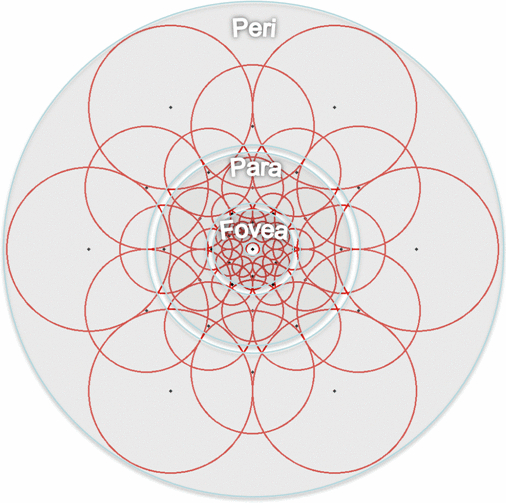
\includegraphics[scale=0.4,keepaspectratio]{circular-sampling-grid.jpg}
    \caption{Illustrazione del pattern di campionamento FREAK simile alla distribuzione delle cellule gangliari retiniche con i corrispondenti campi ricettivi. Ogni cerchio rappresenta un campo ricettivo in cui l'immagine viene levigata con il corrispondente kernel Gaussiano~\cite{6247715}}
    \label{fig:5}
\end{figure}
\noindent La sovrapposizione dei cerchi permette usare meno campi recettivi, poiché viene presa in considerazione come informazione da codificare, esattamente come per l'occhio umano che utilizza una strategia simile. Il descrittore binario, che per brevità chiameremo F, è costruito imponendo una soglia tra le coppie di campi recettivi e i loro Kernel Gaussiani (\ref{eq:1.18}) corrispondenti. \par
\begin{equation}
    {\displaystyle K(u)={\frac {1}{\sqrt {2\pi }}}e^{-{\frac {1}{2}}u^{2}}} \label{eq:1.18}
\end{equation}
\noindent Quindi ogni stringa binaria è composta da DoG rappresentati da un bit (\ref{eq:1.19}).
\begin{equation}
    F=\sum_{0\leq a < N}2^{a}T(P_{a}) \label{eq:1.19}
\end{equation}
\noindent dove \textit{\(P_{a}\)} è la coppia di campi recettivi e N la grandezza del descrittore desiderata e:
\begin{equation}
    T(P_{a})=\begin{cases}
       1 & \text{se \( (I(P_{a}^{r_{1}})-I(P_{a}^{r_{2}}) > 0 \)}  \\
       0 & \text{altrimenti}
    \end{cases}
\end{equation}
\noindent dove \textit{I} è l'intensità. Questa serie di operazioni porta ad avere un descrittore di una certa grandezza e per raffinarlo si seguono i seguenti passi:
\begin{enumerate}
    \item Dai punti corrispondenti estratti si crea una matrice D, in cui ogni riga rappresenta un punto chiave dato da tutte le possibili coppie. Si usano quindi 43 campi recettivi, questo porta ad avere approssimativamente 1000 coppie
    \item Per ogni colonna si calcola la media.
    \item Si ordinano le colonne rispetto alla varianza più alta.
    \item Prendiamo le colonne la cui media è di 0.5 e aggiungiamo a queste le rimanenti colonne che hanno una bassa correlazione con esse.
\end{enumerate}
\noindent Questo passaggio da grossolano a fine definisce la struttura del descrittore. Per mimare i movimenti individuali discontinui dell'occhio, si analizza in diversi step il descrittore. Si inizia l'analisi prendendo i primi 16 bytes che rappresentano l'informazione grossolana, e se la distanza è minore di una soglia si va avanti nella ricerca verso informazioni più fini.
Facendo così si accelera il processo di matching e si eliminano più del 90\% dei candidati.
Per calcolare la rotazione di un punto chiave, si sommano i gradienti locali stimati come nell'algoritmo BRISK.
\noindent Si prende un set \textit{G} di tutte le coppie usate per calcolare i gradienti locali:
\begin{equation}
    O=\frac{1}{M} \sum_{P_{o}\in G}(I(P_{o}^{r_{1}})-I(P_{o}^{r_{2}}))\frac{P_{o}^{r_{1}}-P_{o}^{r_{2}}}{\Vert P_{o}^{r_{1}}-P_{o}^{r_{2}}\Vert}
\end{equation}
\noindent dove M è il numero delle coppie dentro G a e \(P_{o}^{r_{i}}\) è il vettore delle coordinate spaziali in due dimensioni del centro del campo ricettivo.